\documentclass[../main.tex]{subfiles}
\begin{document}

Brown 运动首次到达 $a$ 处的时刻 $T_a=\inf\{t|t\geq0,B(t)=a\}$ 称为 $a$ 的\emph{首中时},而 $M_t=\sup_{0\leq s\leq t}B(s)$ 为 $B(t)$ 在 $[0,t)$ 上的最大值。

显然 $\forall a\geq0$,事件 $\{T_a\leq t\}$ 与 $\{M_t\geq a\}$ 等价。注意到对称性(如图~\ref{fig:8.3.1}),有 $P(B(t)\geq a)=P(T_a\leq t)P(B(t)\geq a|T_a\leq t)+P(T_a\geq t)P(B(t)\geq a|T_a\geq t)=P(T_a\leq t)P(B(t)\geq a|T_a\leq t)=\frac12P(T_a\leq t)$,因此 $P(T_a\leq t)=2P(B(t)\geq a)=2(1-\Phi(\frac a{\sqrt t}))$。

\begin{figure}[!h]
    \centering
    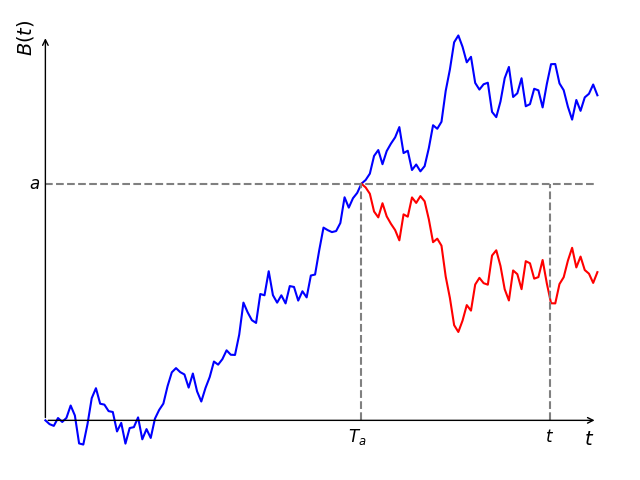
\includegraphics[scale=0.7]{figures/brownian_motion_symmetry.png}
    \caption{Brown 运动在首中时后的对称性}
    \label{fig:8.3.1}
\end{figure}

\begin{proposition}
    粒子从 $0$ 出发,在有限时刻到达 $a$ 的概率为 $1$,即 $P(T_a<+\infty)=1$(具有常返性);但首次到达 $a$ 的平均用时 $\mathrm E(T_a)=+\infty$(具有零常返性)。
\end{proposition}

\end{document}
